% Asset ID: FA22FurtherKinematicsTikZ-002
% Source: Transcript derivation of acceleration as a function of displacement
% Related lesson section: Core Theory; Visual Asset Integration
% Used placeholder:
% [VISUAL PLACEHOLDER: FA22FurtherKinematicsTikZ-002 | Source: Transcript derivation of acceleration as a function of displacement | Insert from tikz/FA22FurtherKinematicsTikZ-002.tex | Purpose: Show the chain-rule derivation of \(a=v\dfrac{dv}{dx}\).]
% Purpose:
% Show the chain-rule derivation of a = v dv/dx and the related identity
% v dv/dx = d/dx(1/2 v^2).

\documentclass[tikz,border=8pt]{standalone}

\usepackage{amsmath}
\usepackage{amssymb}
\usetikzlibrary{arrows.meta, positioning, calc}

\definecolor{Canvas}{HTML}{FAF9F6}
\definecolor{Panel}{HTML}{FFFFF0}
\definecolor{Line}{HTML}{E5E5EA}
\definecolor{Text}{HTML}{2C2C2E}
\definecolor{Gold}{HTML}{C5A059}
\definecolor{Rose}{HTML}{FBEFEF}

\begin{document}

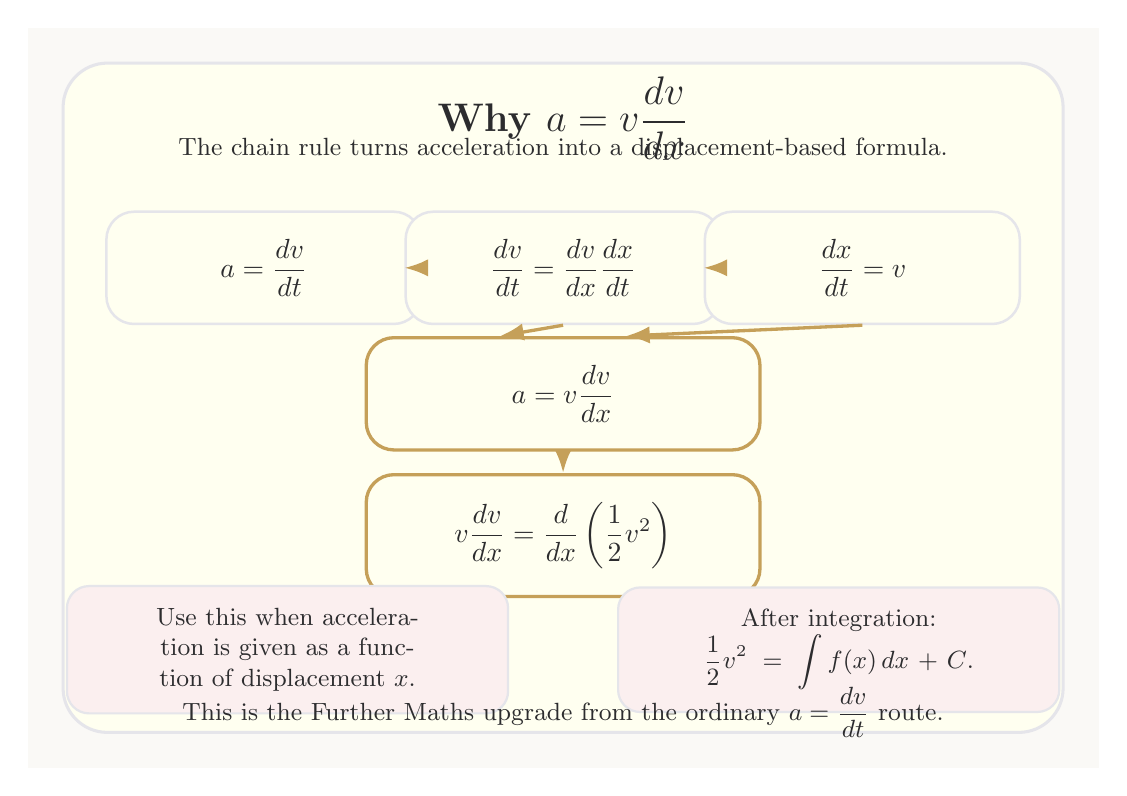
\begin{tikzpicture}[
  font=\sffamily,
  stepbox/.style={
    rounded corners=10pt,
    draw=Line,
    line width=0.9pt,
    fill=Panel,
    align=center,
    text=Text,
    inner xsep=12pt,
    inner ysep=10pt,
    minimum width=4.0cm,
    minimum height=1.1cm
  },
  highlight/.style={
    rounded corners=10pt,
    draw=Gold,
    line width=1.2pt,
    fill=Panel,
    align=center,
    text=Text,
    inner xsep=12pt,
    inner ysep=10pt,
    minimum width=5.0cm,
    minimum height=1.15cm
  },
  note/.style={
    rounded corners=8pt,
    draw=Line,
    line width=0.8pt,
    fill=Rose,
    align=center,
    text=Text,
    inner xsep=10pt,
    inner ysep=8pt,
    font=\small
  },
  arrow/.style={
    -{Latex[length=3mm,width=2.2mm]},
    line width=1.2pt,
    draw=Gold
  }
]

\fill[Canvas] (-6.8,-4.7) rectangle (6.8,4.7);
\draw[Line, line width=1.1pt, rounded corners=16pt, fill=Panel]
  (-6.35,-4.25) rectangle (6.35,4.25);

\node[text=Text, font=\bfseries\Large, align=center] at (0,3.55)
  {Why \(a=v\dfrac{dv}{dx}\)};
\node[text=Text, font=\small, align=center] at (0,3.15)
  {The chain rule turns acceleration into a displacement-based formula.};

\node[stepbox] (s1) at (-3.8,1.65)
  {\(\displaystyle a=\frac{dv}{dt}\)};

\node[stepbox] (s2) at (0,1.65)
  {\(\displaystyle \frac{dv}{dt}
      =
      \frac{dv}{dx}\frac{dx}{dt}\)};

\node[stepbox] (s3) at (3.8,1.65)
  {\(\displaystyle \frac{dx}{dt}=v\)};

\draw[arrow] (s1.east) -- (s2.west);
\draw[arrow] (s2.east) -- (s3.west);

\node[highlight] (final) at (0,0.05)
  {\(\displaystyle a=v\frac{dv}{dx}\)};

\draw[arrow] (s2.south) -- ($(final.north)+(-0.8,0)$);
\draw[arrow] (s3.south) -- ($(final.north)+(0.8,0)$);

\node[highlight] (identity) at (0,-1.75)
  {\(\displaystyle
    v\frac{dv}{dx}
    =
    \frac{d}{dx}\left(\frac{1}{2}v^2\right)
  \)};

\draw[arrow] (final.south) -- (identity.north);

\node[note, text width=4.9cm] at (-3.5,-3.2)
  {Use this when acceleration is given as a function of displacement \(x\).};

\node[note, text width=4.9cm] at (3.5,-3.2)
  {After integration: \(\displaystyle \frac12v^2=\int f(x)\,dx+C\).};

\node[text=Text, font=\small, align=center] at (0,-4.0)
  {This is the Further Maths upgrade from the ordinary \(a=\dfrac{dv}{dt}\) route.};

\end{tikzpicture}

\end{document}
